%package list
\documentclass{article}
\usepackage[top=3cm, bottom=3cm, outer=3cm, inner=3cm]{geometry}
\usepackage{multicol}
\usepackage{graphicx}
\usepackage{url}
%\usepackage{cite}
\usepackage{hyperref}
\usepackage{array}
%\usepackage{multicol}
\newcolumntype{x}[1]{>{\centering\arraybackslash\hspace{0pt}}p{#1}}
\usepackage{natbib}
\usepackage{pdfpages}
\usepackage{multirow}
\usepackage[normalem]{ulem}
\useunder{\uline}{\ul}{}
\usepackage{svg}
\usepackage{xcolor}
\usepackage{listings}
\lstdefinestyle{ascii-tree}{
    literate={├}{|}1 {─}{--}1 {└}{+}1 
  }
\lstset{basicstyle=\ttfamily,
  showstringspaces=false,
  commentstyle=\color{red},
  keywordstyle=\color{blue}
}
%\usepackage{booktabs}
\usepackage{caption}
\usepackage{subcaption}
\usepackage{float}
\usepackage{array}

\newcolumntype{M}[1]{>{\centering\arraybackslash}m{#1}}
\newcolumntype{N}{@{}m{0pt}@{}}


%%%%%%%%%%%%%%%%%%%%%%%%%%%%%%%%%%%%%%%%%%%%%%%%%%%%%%%%%%%%%%%%%%%%%%%%%%%%
%%%%%%%%%%%%%%%%%%%%%%%%%%%%%%%%%%%%%%%%%%%%%%%%%%%%%%%%%%%%%%%%%%%%%%%%%%%%
\newcommand{\itemEmail}{- Wiliam Herderson Choquehuanca Berna}
\newcommand{\itemStudent}{ - Ajra Huacso Jeans Anthony}
\newcommand{\itemCourse}{Programación Web 2}
\newcommand{\itemCourseCode}{20232208}
\newcommand{\itemSemester}{I}
\newcommand{\itemUniversity}{Universidad Nacional de San Agustín de Arequipa}
\newcommand{\itemFaculty}{Facultad de Ingeniería de Producción y Servicios}
\newcommand{\itemDepartment}{Departamento Académico de Ingeniería de Sistemas e Informática}
\newcommand{\itemSchool}{Escuela Profesional de Ingeniería de Sistemas}
\newcommand{\itemAcademic}{2024 - A}
\newcommand{\itemInput}{Del 28 Abril 2024}
\newcommand{\itemOutput}{Al 3 Mayo 2024}
\newcommand{\itemPracticeNumber}{01}
\newcommand{\itemTheme}{DOCKER}
%%%%%%%%%%%%%%%%%%%%%%%%%%%%%%%%%%%%%%%%%%%%%%%%%%%%%%%%%%%%%%%%%%%%%%%%%%%%
%%%%%%%%%%%%%%%%%%%%%%%%%%%%%%%%%%%%%%%%%%%%%%%%%%%%%%%%%%%%%%%%%%%%%%%%%%%%

\usepackage[english,spanish]{babel}
\usepackage[utf8]{inputenc}
\AtBeginDocument{\selectlanguage{spanish}}
\renewcommand{\figurename}{Figura}
\renewcommand{\refname}{Referencias}
\renewcommand{\tablename}{Tabla} %esto no funciona cuando se usa babel
\AtBeginDocument{%
	\renewcommand\tablename{Tabla}
}

\usepackage{fancyhdr}
\pagestyle{fancy}
\fancyhf{}
\setlength{\headheight}{30pt}
\renewcommand{\headrulewidth}{1pt}
\renewcommand{\footrulewidth}{1pt}
\fancyhead[L]{\raisebox{-0.2\height}{
\includegraphics[width=3cm]{img/logo_episunsa.png}}}
\fancyhead[C]{\fontsize{7}{7}\selectfont	\itemUniversity \\ \itemFaculty \\ \itemDepartment \\ \itemSchool \\ \textbf{\itemCourse}}
\fancyhead[R]{\raisebox{-0.2\height}{
\includegraphics[width=1.2cm]{img/logo_abet}}}
\fancyfoot[L]{Estudiante Juan Perez Perez}
\fancyfoot[C]{\itemCourse}
\fancyfoot[R]{Página \thepage}

% para el codigo fuente
\usepackage{listings}
\usepackage{color, colortbl}
\definecolor{dkgreen}{rgb}{0,0.6,0}
\definecolor{gray}{rgb}{0.5,0.5,0.5}
\definecolor{mauve}{rgb}{0.58,0,0.82}
\definecolor{codebackground}{rgb}{0.95, 0.95, 0.92}
\definecolor{tablebackground}{rgb}{0.8, 0, 0}

\lstset{frame=tb,
	language=bash,
	aboveskip=3mm,
	belowskip=3mm,
	showstringspaces=false,
	columns=flexible,
	basicstyle={\small\ttfamily},
	numbers=none,
	numberstyle=\tiny\color{gray},
	keywordstyle=\color{blue},
	commentstyle=\color{dkgreen},
	stringstyle=\color{mauve},
	breaklines=true,
	breakatwhitespace=true,
	tabsize=3,
	backgroundcolor= \color{codebackground},
}

\begin{document}
	
	\vspace*{10px}
	
	\begin{center}	
		\fontsize{17}{17} \textbf{ Informe de Laboratorio \itemPracticeNumber}
	\end{center}
	\centerline{\textbf{\Large Tema: \itemTheme}}
	%\vspace*{0.5cm}	

	\begin{flushright}
		\begin{tabular}{|M{2.5cm}|N|}
			\hline 
			\rowcolor{tablebackground}
			\color{white} \textbf{Nota}  \\
			\hline 
			     \\[30pt]
			\hline 			
		\end{tabular}
	\end{flushright}	

	\begin{table}[H]
		\begin{tabular}{|x{4.7cm}|x{4.8cm}|x{4.8cm}|}
			\hline 
			\rowcolor{tablebackground}
			\color{white} \textbf{Estudiante} & \color{white}\textbf{Escuela}  & \color{white}\textbf{Asignatura}   \\
			\hline 
			{\itemStudent \par \itemEmail} & \itemSchool & {\itemCourse \par Semestre: \itemSemester \par Código: \itemCourseCode}     \\
			\hline 			
		\end{tabular}
	\end{table}		
	
	\begin{table}[H]
		\begin{tabular}{|x{4.7cm}|x{4.8cm}|x{4.8cm}|}
			\hline 
			\rowcolor{tablebackground}
			\color{white}\textbf{Laboratorio} & \color{white}\textbf{Tema}  & \color{white}\textbf{Duración}   \\
			\hline 
			\itemPracticeNumber & \itemTheme & 04 horas   \\
			\hline 
		\end{tabular}
	\end{table}
	
	\begin{table}[H]
		\begin{tabular}{|x{4.7cm}|x{4.8cm}|x{4.8cm}|}
			\hline 
			\rowcolor{tablebackground}
			\color{white}\textbf{Semestre académico} & \color{white}\textbf{Fecha de inicio}  & \color{white}\textbf{Fecha de entrega}   \\
			\hline 
			\itemAcademic & \itemInput &  \itemOutput  \\
			\hline 
		\end{tabular}
	\end{table}
	
	\section{ENTREGABLE 1: Capturas de la Instalación y subida del proyecto}
\item INTEGRANTES DEL GRUPO:
\item - AJRA HUACSO JEANS ANTHONY
\item - WILLIAM HERDERSON CHOQUEHUANCA BERNA
        
	\begin{itemize}		
    \item 
    CAPTURAS DE LA INSTALACIÓN Y SUBIDA DEL PROYECTO
    \end{itemize}
        
\begin{flushleft}
\begin{verbatim}
En primer lugar, lo que hacemos es crear un nuevo contenedor abriendo un total de tres 
puertos, esto haciendo una copia local de la imagen de Ubuntu, con el comando que se
muestra a continuación, el proceso también se encuentra dentro del mismo.

Esto nos permite el utilizar el mismo contenedor, y en este mismo poder isntalar todas
las dependencias de nuestro proyecto para que tenga un funcionamiento de manera local, 
lo que nos permitira el obserbar nuestro proyecto del semestre pasado.

\end{verbatim}
\end{flushleft}

\begin{figure}[h]
    \centering
    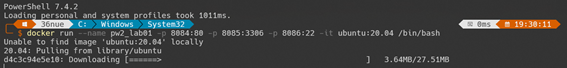
\includegraphics[width=1\textwidth]{img/1.png}
    \label{fig:imagen}
\end{figure}

\begin{flushleft}
\begin{verbatim}





Después de eso, lo que hacemos es usar el comando “apt-get update” para poder realizar
los comandos que nos serán útiles más adelante:
\end{verbatim}
\end{flushleft}

\begin{figure}[h]
    \centering
    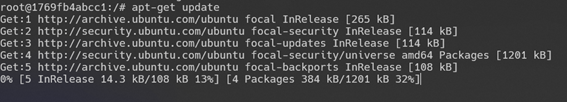
\includegraphics[width=1\textwidth]{img/2.png}
    \label{fig:imagen}
\end{figure}


\begin{flushleft}
\begin{verbatim}


Seguidamente usamos el comando que se muestra a continuación para poder instalar el
apache dentro de nuestro contenedor:
\end{verbatim}
\end{flushleft}

\begin{figure}[h]
    \centering
    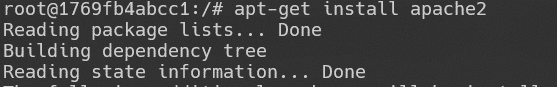
\includegraphics[width=1\textwidth]{img/3.png}
    \label{fig:imagen}
\end{figure}



\begin{flushleft}
\begin{verbatim}



Usamos el mismo comando, cambiando en este caso el nombre del APACHE por SSH para 
poder utilizarlo al momento de lanzar nuestro proyecto:
\end{verbatim}
\end{flushleft}

\begin{figure}[h]
    \centering
    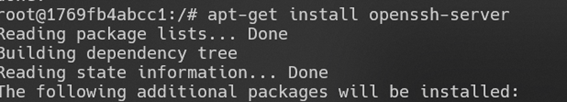
\includegraphics[width=1\textwidth]{img/4.png}
    \label{fig:imagen}
\end{figure}

\begin{flushleft}
\begin{verbatim}








Ahora en este caso utilizaremos el mismo comando para MariaDB en este caso, para 
poder utilizar nuestras bases de datos dentro de nuestro contenedor de Docker, 
que es donde podremos colocar nuestro proyecto.
\end{verbatim}
\end{flushleft}

\begin{figure}[h]
    \centering
    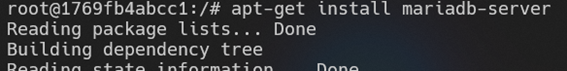
\includegraphics[width=1\textwidth]{img/5.png}
    \label{fig:imagen}
\end{figure}




\begin{flushleft}
\begin{verbatim}



Asimismo, configuramos el perl dentro de nuestro servidor local para poder dar 
funcionalidad a nuestros scripts cgi de nuestro proyecto.
\end{verbatim}
\end{flushleft}

\begin{figure}[h]
    \centering
    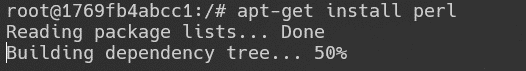
\includegraphics[width=1\textwidth]{img/6.png}
    \label{fig:imagen}
\end{figure}



\begin{flushleft}
\begin{verbatim}



Por último, instalamos git para poder clonar directamente nuestro repositorio
del proyecto dentro de los espacios del servidor que estamos utilizando
\end{verbatim}
\end{flushleft}

\begin{figure}[h]
    \centering
    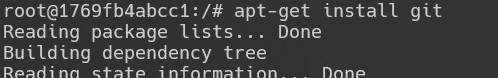
\includegraphics[width=1\textwidth]{img/7.png}
    \label{fig:imagen}
\end{figure}


\begin{flushleft}
\begin{verbatim}










Con ello resuelto, lo que hacemos es buscar la dirección del directorio HTML, y
posicionarnos en el directorio que lo contiene, porque en ese será el lugar en 
el que clonaremos nuestro repositorio para poder observar nuestro proyecto pasado.
En ese mismo lugar usamos el comando “git clone 
https://github.com/RyanValdivia/pweb1-trabajoFinal” para poder clonar el proyecto
de nuestro proyecto
\end{verbatim}
\end{flushleft}

\begin{figure}[h]
    \centering
    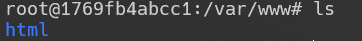
\includegraphics[width=1\textwidth]{img/8.png}
    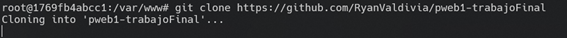
\includegraphics[width=1\textwidth]{img/9.png}
    \label{fig:imagen}
\end{figure}





\begin{flushleft}
\begin{verbatim}







Después de esto, borramos el directorio de HMTL y en vez de ello, cambiamos 
el nombre de nuestro proyecto copiado desde github a “Html” esto nos permitirá
el poder visualizar nuestra página de manera directa:
\end{verbatim}
\end{flushleft}

\begin{figure}[h]
    \centering
    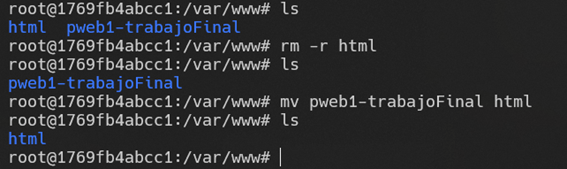
\includegraphics[width=1\textwidth]{img/10.png}
    \label{fig:imagen}
\end{figure}




\begin{flushleft}
\begin{verbatim}











Ahora lo que procede es el poder configurar la base de datos con la información
que teníamos en nuestro directorio: Esto lo usamos utilizando el comando “mysql 
-u root -p” después de haber inicializado el sql dentro de nuestro contenedor, 
esto nos permitirá ingresar al root de la base de datos, y para poder importar 
nuestras tablas, primero creamos una base de datos general, en este caso con el
nombre de “biblioteca” y después importamos con el comando “source” para poder
importar nuestra información:
\end{verbatim}
\end{flushleft}

\begin{figure}[h]
    \centering
    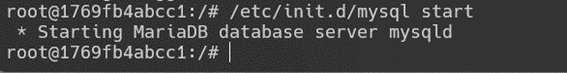
\includegraphics[width=1\textwidth]{img/11.png}
    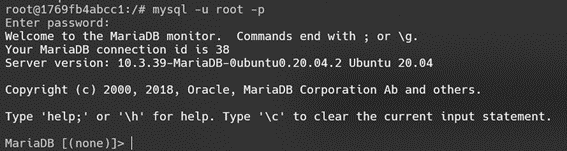
\includegraphics[width=1\textwidth]{img/12.png}
    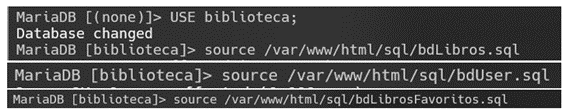
\includegraphics[width=1\textwidth]{img/13.png}
    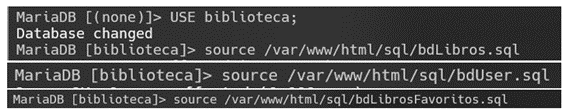
\includegraphics[width=1\textwidth]{img/13.png}    
    \label{fig:imagen}
\end{figure}


\begin{flushleft}
    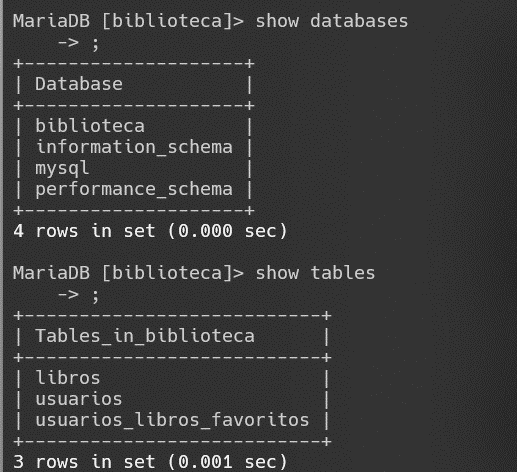
\includegraphics[width=1\textwidth]{img/14.png}
\begin{verbatim}


Ahora con esto, podemos dar funcionalidad a nuestra página final, pero solo nos 
queda el iniciar el server apache y el ssh, esto se hace a continuación:
\end{verbatim}
\end{flushleft}

\begin{figure}[h]
    \centering
    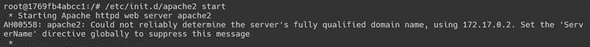
\includegraphics[width=1\textwidth]{img/15.png}
    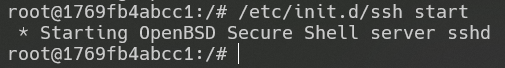
\includegraphics[width=1\textwidth]{img/16.png}
    
    
    \label{fig:imagen}
\end{figure}






\begin{flushleft}
\begin{verbatim}


Esto es todo lo que se necesita para poder correr nuestro proyecto dentro de docker,
y para poder visualizarlo simplmente obserbamos los puertos que se utilizan dentro
de nuestro desktop, en este caso usamos el puerto 8084 para poder visualizar nuestro
proyecto, teniendo lo siguiente:
\end{verbatim}
\end{flushleft}

\begin{figure}[h]
    \centering
    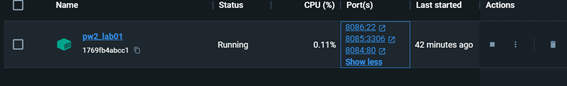
\includegraphics[width=1\textwidth]{img/17.png}    
    \label{fig:imagen}
\end{figure}


\begin{itemize}		
    \item 
    CAPTURAS DE LA INICIALIZACIÓN DE AMBOS PROYECTOS:
\end{itemize}

\begin{itemize}		
    \item 
    PROYECTO 1:
\end{itemize}
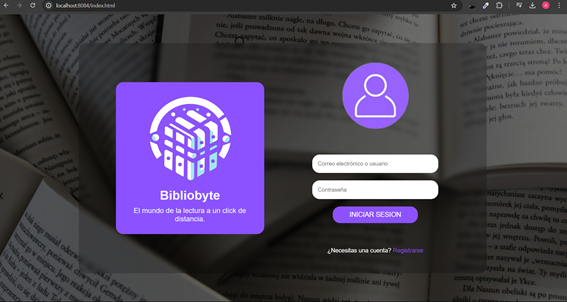
\includegraphics[width=1\textwidth]{img/18.png} 
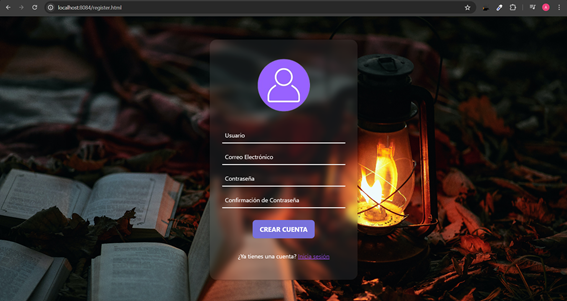
\includegraphics[width=1\textwidth]{img/19.png} 
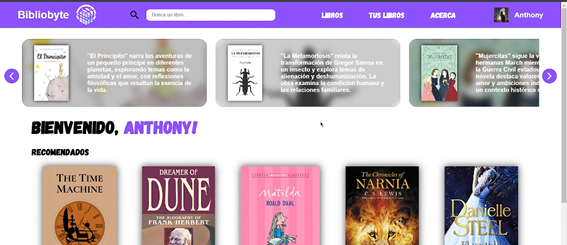
\includegraphics[width=1\textwidth]{img/20.png} 
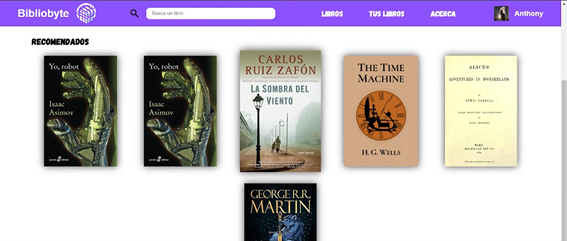
\includegraphics[width=1\textwidth]{img/21.png} 


\begin{itemize}		
    \item 
    PROYECTO 2:
\end{itemize}
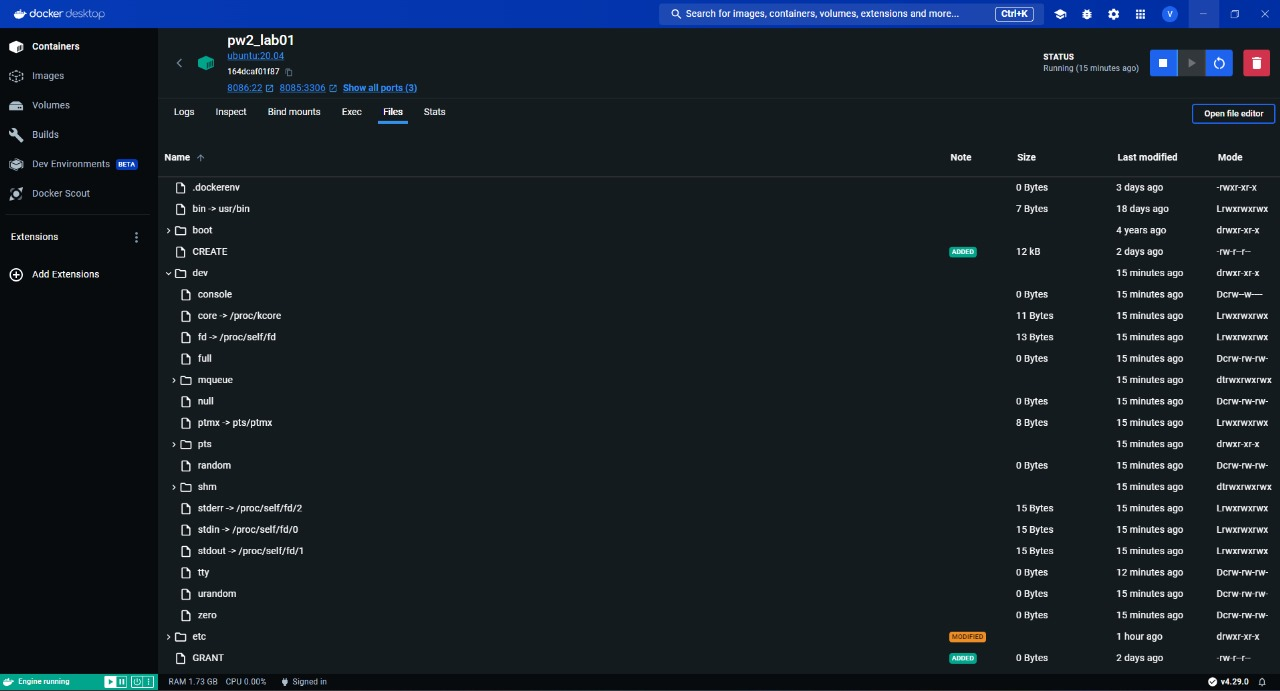
\includegraphics[width=1\textwidth]{img/22.jpeg} 
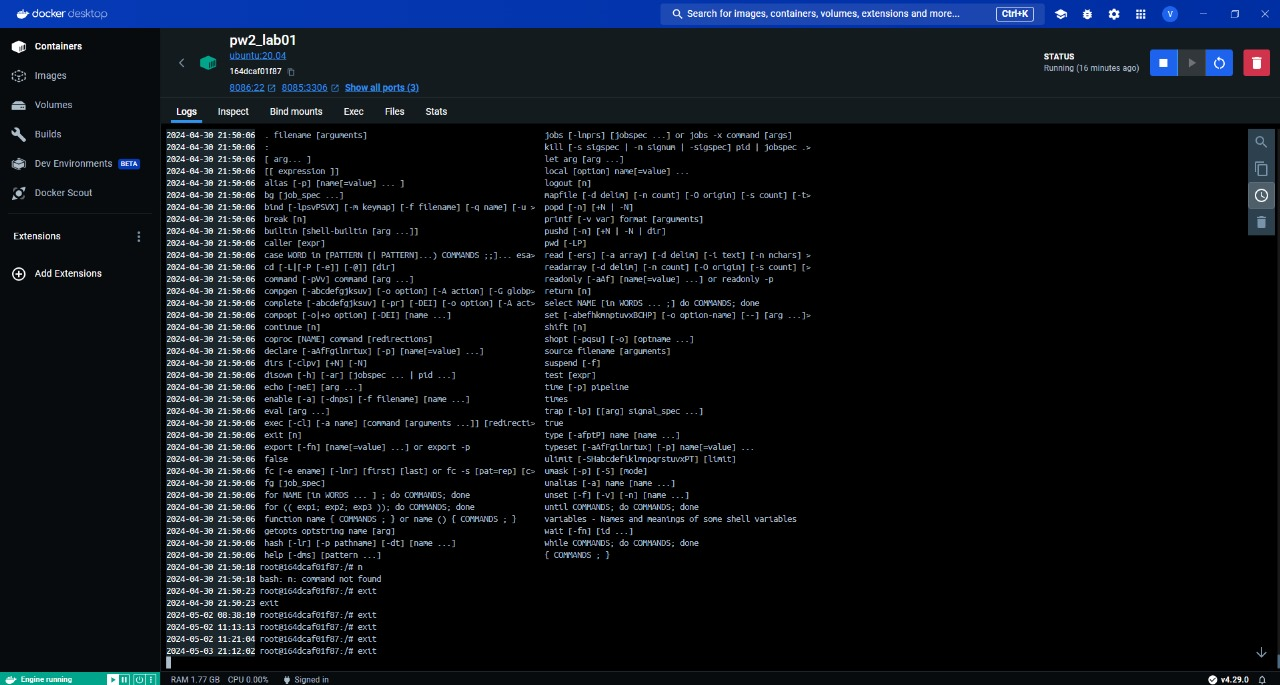
\includegraphics[width=1\textwidth]{img/23.jpeg} 
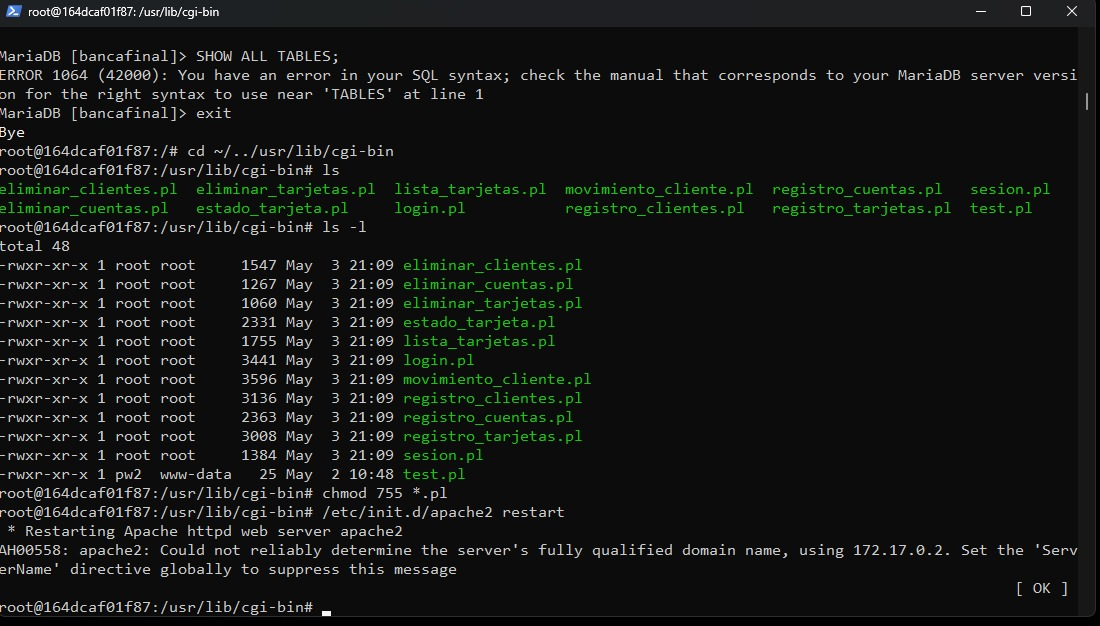
\includegraphics[width=1\textwidth]{img/24.jpeg} 
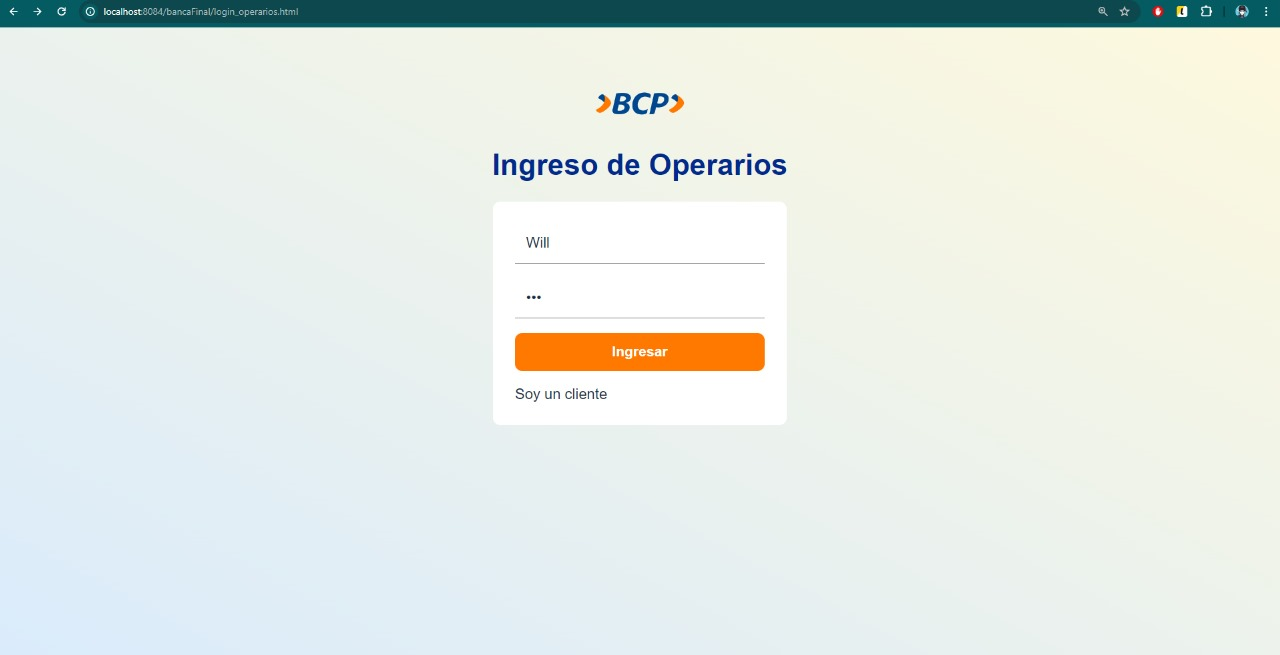
\includegraphics[width=1\textwidth]{img/25.jpeg} 




\section{ENTREGABLE 2: links de los materiales}
    \begin{itemize}	
    
    \item Link Gitlab (Informe en Latex): https://gitlab.com/nuevo637/Informe1-Programacion-Web
    
    \item Link del video(Flip) PROYECTO 1: https://flip.com/s/FDwHFDMD1HLj
    
    \item Link del video(Flip) PROYECTO 2: https://flip.com/s/_Zuzz8ujFS8F
    
    \item Link de Dockerhub PROYECTO 1: https://hub.docker.com/repository/docker/anthonyajra/proyectoweb/general
    
    \item Comando de descarga de Dockerhub PROYECTO 1:  docker pull anthonyajra/proyectoweb
    
    \item Link de Dockerhub PROYECTO 2: https://hub.docker.com/repository/docker/velmork/pw2_lab01/general
    
    \item Comando de descarga de Dockerhub PROYECTO 2: docker pull velmork/pw2_lab01
\end{itemize}











   
\section{Referencias}
\begin{itemize}			
	\item \url{hhttps://www.docker.com/}
\end{itemize}	
	
%\clearpage
%\bibliographystyle{apalike}
%\bibliographystyle{IEEEtranN}
%\bibliography{bibliography}
			
\end{document}